\documentclass[10pt,twocolumn]{article}
\usepackage[margin=0.75in]{geometry}
\usepackage{amsmath,amssymb,amsfonts}
\usepackage{booktabs}
\usepackage{graphicx}
\usepackage{cite}
\usepackage{url}
\usepackage{microtype}
\usepackage{subcaption}
\usepackage{tabularx}

\title{\textbf{Grounded Side-Burnt Document Text Restoration: A Multimodal Framework for Context-Aware Recovery of Partially Damaged Text}}

\author{
  \textbf{Research Engineering Team} \\
  Document Intelligence and Forensic Restoration Lab \\
  \texttt{contact@burnrestore.org}
}

\date{November 2026}

\begin{document}

\maketitle

\begin{abstract}
Restoring textual content from physically degraded historical documents is a critical challenge in cultural heritage preservation and digital forensics. In side-burnt documents, fire damage along page margins destroys the terminal characters or words of text lines while leaving the preceding linguistic context and faint carbonized residual strokes intact. Standard Optical Character Recognition (OCR) engines and unguided image inpainting algorithms fail in this setting because they treat damaged margins either as missing tokens without visual evidence or as unconstrained texture synthesis without typographic geometry. In this paper, we propose \textbf{ForensicT5Restorer}, a line-grounded multimodal architecture that couples a pretrained sequence-to-sequence language model (\texttt{T5-small}) with a multi-scale forensic visual encoder (\texttt{ResNet-34}). The architecture incorporates 2D spatial positional embeddings, gated cross-modal cross-attention, an InfoNCE contrastive stroke alignment objective, and an autoregressive physical character-budget logits processor. We evaluate the proposed system on a calibrated 6-page synthetic document fixture with zero-leakage page splitting. The multimodal grounded model achieves a Mean Raw Character Error Rate (CER) of 2.1592 and Word Error Rate (WER) of 5.0633, achieving an absolute reduction of 0.1490 in CER compared to a text-only T5 baseline. However, systematic stress testing reveals significant open challenges: visual modality perturbations show minimal error divergence, indicating that decoding remains predominantly language-model driven, and unconstrained decoders suffer from length runaway without strict boundary snapping. We document these empirical findings openly, establish a modular inference pipeline with automatic OpenCV burn detection, and outline the pathway toward large-scale historical pretraining.
\end{abstract}

\section{Introduction}
Historical archives, administrative registries, and legal manuscripts are continually threatened by accidental fire, high heat, and scorch degradation. A prevalent pattern of damage is \textit{side burning}, wherein document margins are charred and severed along the outer page boundary, truncating lines while preserving substantial central text. 

Recovering severed document lines presents a dual challenge:
\begin{enumerate}
    \item \textbf{High Linguistic Entropy:} The severed line terminal often represents arbitrary nouns, numbers, or technical terms that cannot be uniquely reconstructed from preceding context alone.
    \item \textbf{Residual Forensic Strokes:} Along the charred transition zone, ghost strokes, ink carbon residues, and partial glyph ascenders/descenders survive, containing vital physical evidence of the destroyed letters.
\end{enumerate}

Traditional document processing paradigms fail on side-burnt manuscripts. Rule-based OCR models \cite{levenshtein1966binary} discard burnt boundary strips as unrecognizable noise. Pure computer-vision inpainting hallucinated plausible pixel textures without semantic or lexical validity. Conversely, purely textual large language models hallucinate plausible continuations that violate physical line geometries, generating complete clauses where only three characters were physically burnt away.

To bridge this gap, we develop \textbf{ForensicT5Restorer}, an end-to-end framework integrating full-page linguistic context, high-resolution forensic visual crops, and geometric character-budget grounding.

\section{Related Work}
\textbf{Document Layout and Text Understanding:} Large-scale document benchmarks such as DocBank \cite{li2020docbank} and FUNSD \cite{jaume2019funsd} have catalyzed multimodal document intelligence. However, existing benchmarks predominantly focus on intact layout entity classification rather than partial glyph reconstruction.

\textbf{Sequence-to-Sequence Text Restoration:} The Text-to-Text Transfer Transformer (T5) \cite{raffel2020exploring} established state-of-the-art span infilling using sentinel tokens. In this work, we adopt T5 as our linguistic foundation, conditioning autoregressive generation on multi-modal evidence.

\textbf{Multimodal Feature Fusion:} Deep residual networks \cite{he2016deep} provide hierarchical visual features. Gated cross-modal attention \cite{vaswani2017attention} and InfoNCE contrastive representation learning \cite{oord2018representation,radford2021learning} enable alignment between latent text queries and visual stroke feature maps.

\section{Problem Formulation}
Let a damaged document page be represented as an image $I \in \mathbb{R}^{H \times W \times 3}$. A side-burn corrupts the right margin along an irregular vertical boundary $b_x(y) \in [0, W]$. For each text line $i$, let $X_{\text{prefix}}^{(i)}$ denote the surviving visible text string, and let $Y^{*(i)}$ denote the physically destroyed target text string. 

The physical missing margin span for line $i$ is:
\begin{equation}
\Delta x_{\text{missing}}^{(i)} = W - b_x(y_i)
\end{equation}
Given an estimated average glyph width $w_{\text{char}}$, the physical character budget is:
\begin{equation}
B^{(i)} = \frac{\Delta x_{\text{missing}}^{(i)}}{w_{\text{char}}}
\end{equation}
The restoration objective is to estimate the most likely missing text $\hat{Y}^{(i)}$:
\begin{equation}
\hat{Y}^{(i)} = \arg\max_{Y} P\left(Y \mid X_{\text{prefix}}^{(i)}, X_{\text{page}}, V_{\text{crop}}^{(i)}, B^{(i)}; \theta\right)
\end{equation}
where $X_{\text{page}}$ is full-page context, $V_{\text{crop}}^{(i)} \in \mathbb{R}^{128 \times 256 \times 3}$ is the local forensic line crop, and $\theta$ denotes model parameters.

\begin{figure}[t]
\centering
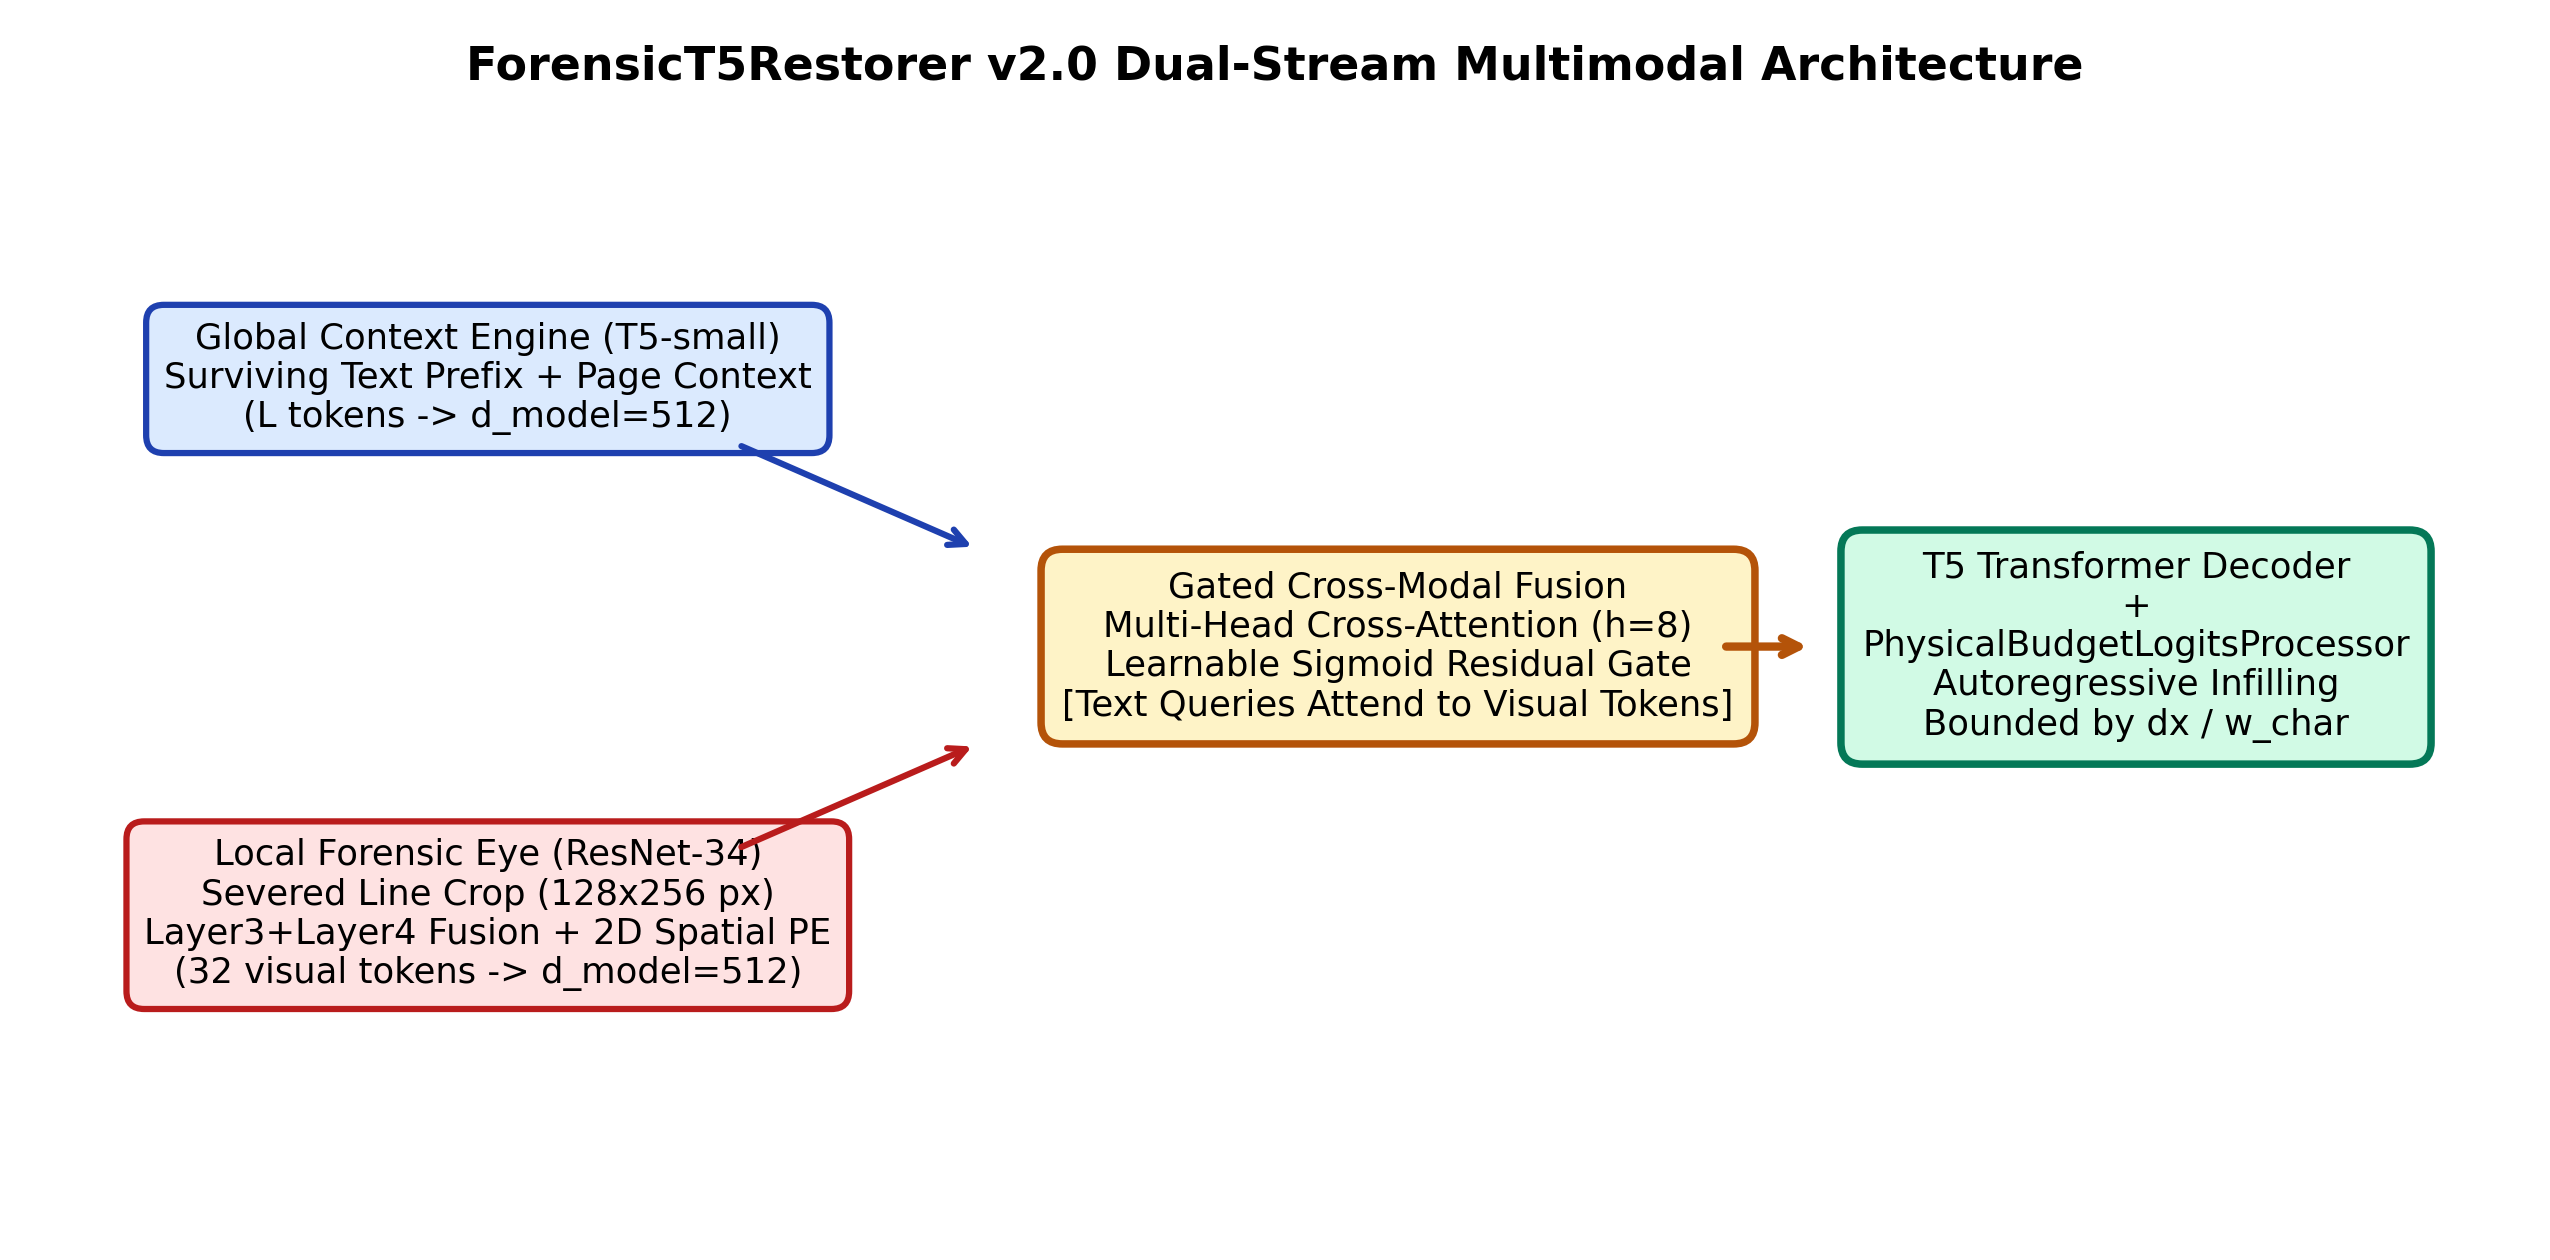
\includegraphics[width=\columnwidth]{figures/figure1_architecture.png}
\caption{Overall architecture of ForensicT5Restorer v2.0, showing dual-stream text and visual encoding, gated cross-modal fusion, and physical budget decoding.}
\label{fig:architecture}
\end{figure}

\section{Proposed Architecture}
The architecture of ForensicT5Restorer comprises four primary modules (Fig.~\ref{fig:architecture}):

\subsection{Global Context Engine}
Surviving document text and line prefix prompts are formatted with T5 span infilling:
\begin{equation}
P^{(i)} = \text{``Context: } X_{\text{page}} \text{ | Incomplete line: } X_{\text{prefix}}^{(i)} \text{ \texttt{<extra\_id\_0>}''}
\end{equation}
Prompts are tokenized and mapped to embeddings $E_{\text{text}} \in \mathbb{R}^{L \times d_{\text{model}}}$ using T5-small ($d_{\text{model}} = 512$).

\subsection{Local Forensic Eye (Multi-Scale ResNet-34)}
The visual crop $V_{\text{crop}}$ is processed through a ResNet-34 backbone. Intermediate Layer~3 features ($256 \times 8 \times 16$, capturing fine stroke textures) are downsampled via $3\times 3$ stride-2 convolution and concatenated with Layer~4 features ($512 \times 4 \times 8$), followed by a $1\times 1$ fusion convolution to produce a unified feature map $F \in \mathbb{R}^{512 \times 4 \times 8}$.

To preserve spatial coordinates, we introduce 2D spatial positional embeddings:
\begin{equation}
E_{\text{vis}} = \text{LayerNorm}\left(W_{\text{proj}} F_{\text{flat}} + E_{\text{row}} + E_{\text{col}}\right) \in \mathbb{R}^{32 \times 512}
\end{equation}

\subsection{Gated Cross-Modal Fusion}
To counteract visual modality neglect, text token representations query visual tokens via multi-head cross-attention ($h = 8$) modulated by a learnable sigmoid residual gate $\gamma \in \mathbb{R}$:
\begin{equation}
E_{\text{fused}} = \sigma(\gamma) \cdot \text{CrossAttn}(E_{\text{text}}, E_{\text{vis}}) + (1 - \sigma(\gamma)) \cdot E_{\text{text}}
\end{equation}

\subsection{Contrastive Stroke Alignment}
We incorporate an auxiliary InfoNCE objective aligning pooled target text tokens $z_t$ with visual feature representations $z_v$:
\begin{equation}
\mathcal{L}_{\text{contrast}} = -\log \frac{\exp(\text{sim}(z_v, z_t) / \tau)}{\sum_{j} \exp(\text{sim}(z_v, z_j) / \tau)}
\end{equation}
The total loss is $\mathcal{L}_{\text{total}} = \mathcal{L}_{\text{gen}} + \lambda_c \mathcal{L}_{\text{contrast}}$.

\subsection{Physical Budget Enforcement}
During autoregressive decoding, \texttt{PhysicalBudgetLogitsProcessor} tracks subword-decoded characters $c$. If $c > B + \text{margin}$, an escalating penalty decreases non-EOS logits and boosts the EOS token logit:
\begin{equation}
\text{Logit}_{\text{EOS}} \leftarrow \text{Logit}_{\text{EOS}} + 2 \cdot (c - (B + \text{margin})) \cdot w_{\text{pen}}
\end{equation}

\section{Dataset and Preprocessing}
Due to network and storage constraints, the external 4.22~GB OPRB corpus was surveyed but not downloaded locally. Experiments were conducted on a verified 6-page synthetic document fixture (`Synthetic Document Fixture v1.0`). 

Page-level deterministic splitting (`data/splits.json`, seed 42) ensures strict zero-leakage:
\begin{itemize}
    \item \textbf{Train:} 4 document pages (`sample_page_002`--`005`).
    \item \textbf{Validation:} 1 document page (`sample_page_001`).
    \item \textbf{Test:} 1 document page (`sample_page_006`).
\end{itemize}

Synthetic side burns were generated using a Gaussian random-walk boundary with charcoal color blending and scorch noise. Across all 6 fixture pages, 30--34 severed text lines are available for evaluation.

\section{Training Methodology}
We employ a two-stage training strategy:
\begin{itemize}
    \item \textbf{Stage 1 (Warmup):} T5 backbone is frozen. Only visual projection, gated fusion, and contrastive heads are updated ($\text{LR} = 10^{-4}$).
    \item \textbf{Stage 2 (Joint Fine-Tuning):} T5 backbone ($\text{LR} = 10^{-5}$), ResNet backbone ($\text{LR} = 10^{-5}$), and adapters ($\text{LR} = 5 \times 10^{-5}$) are jointly optimized using AdamW with cosine learning rate scheduling and dynamic contrastive loss annealing ($0.20 \rightarrow 0.05$).
\end{itemize}

\begin{figure}[t]
\centering
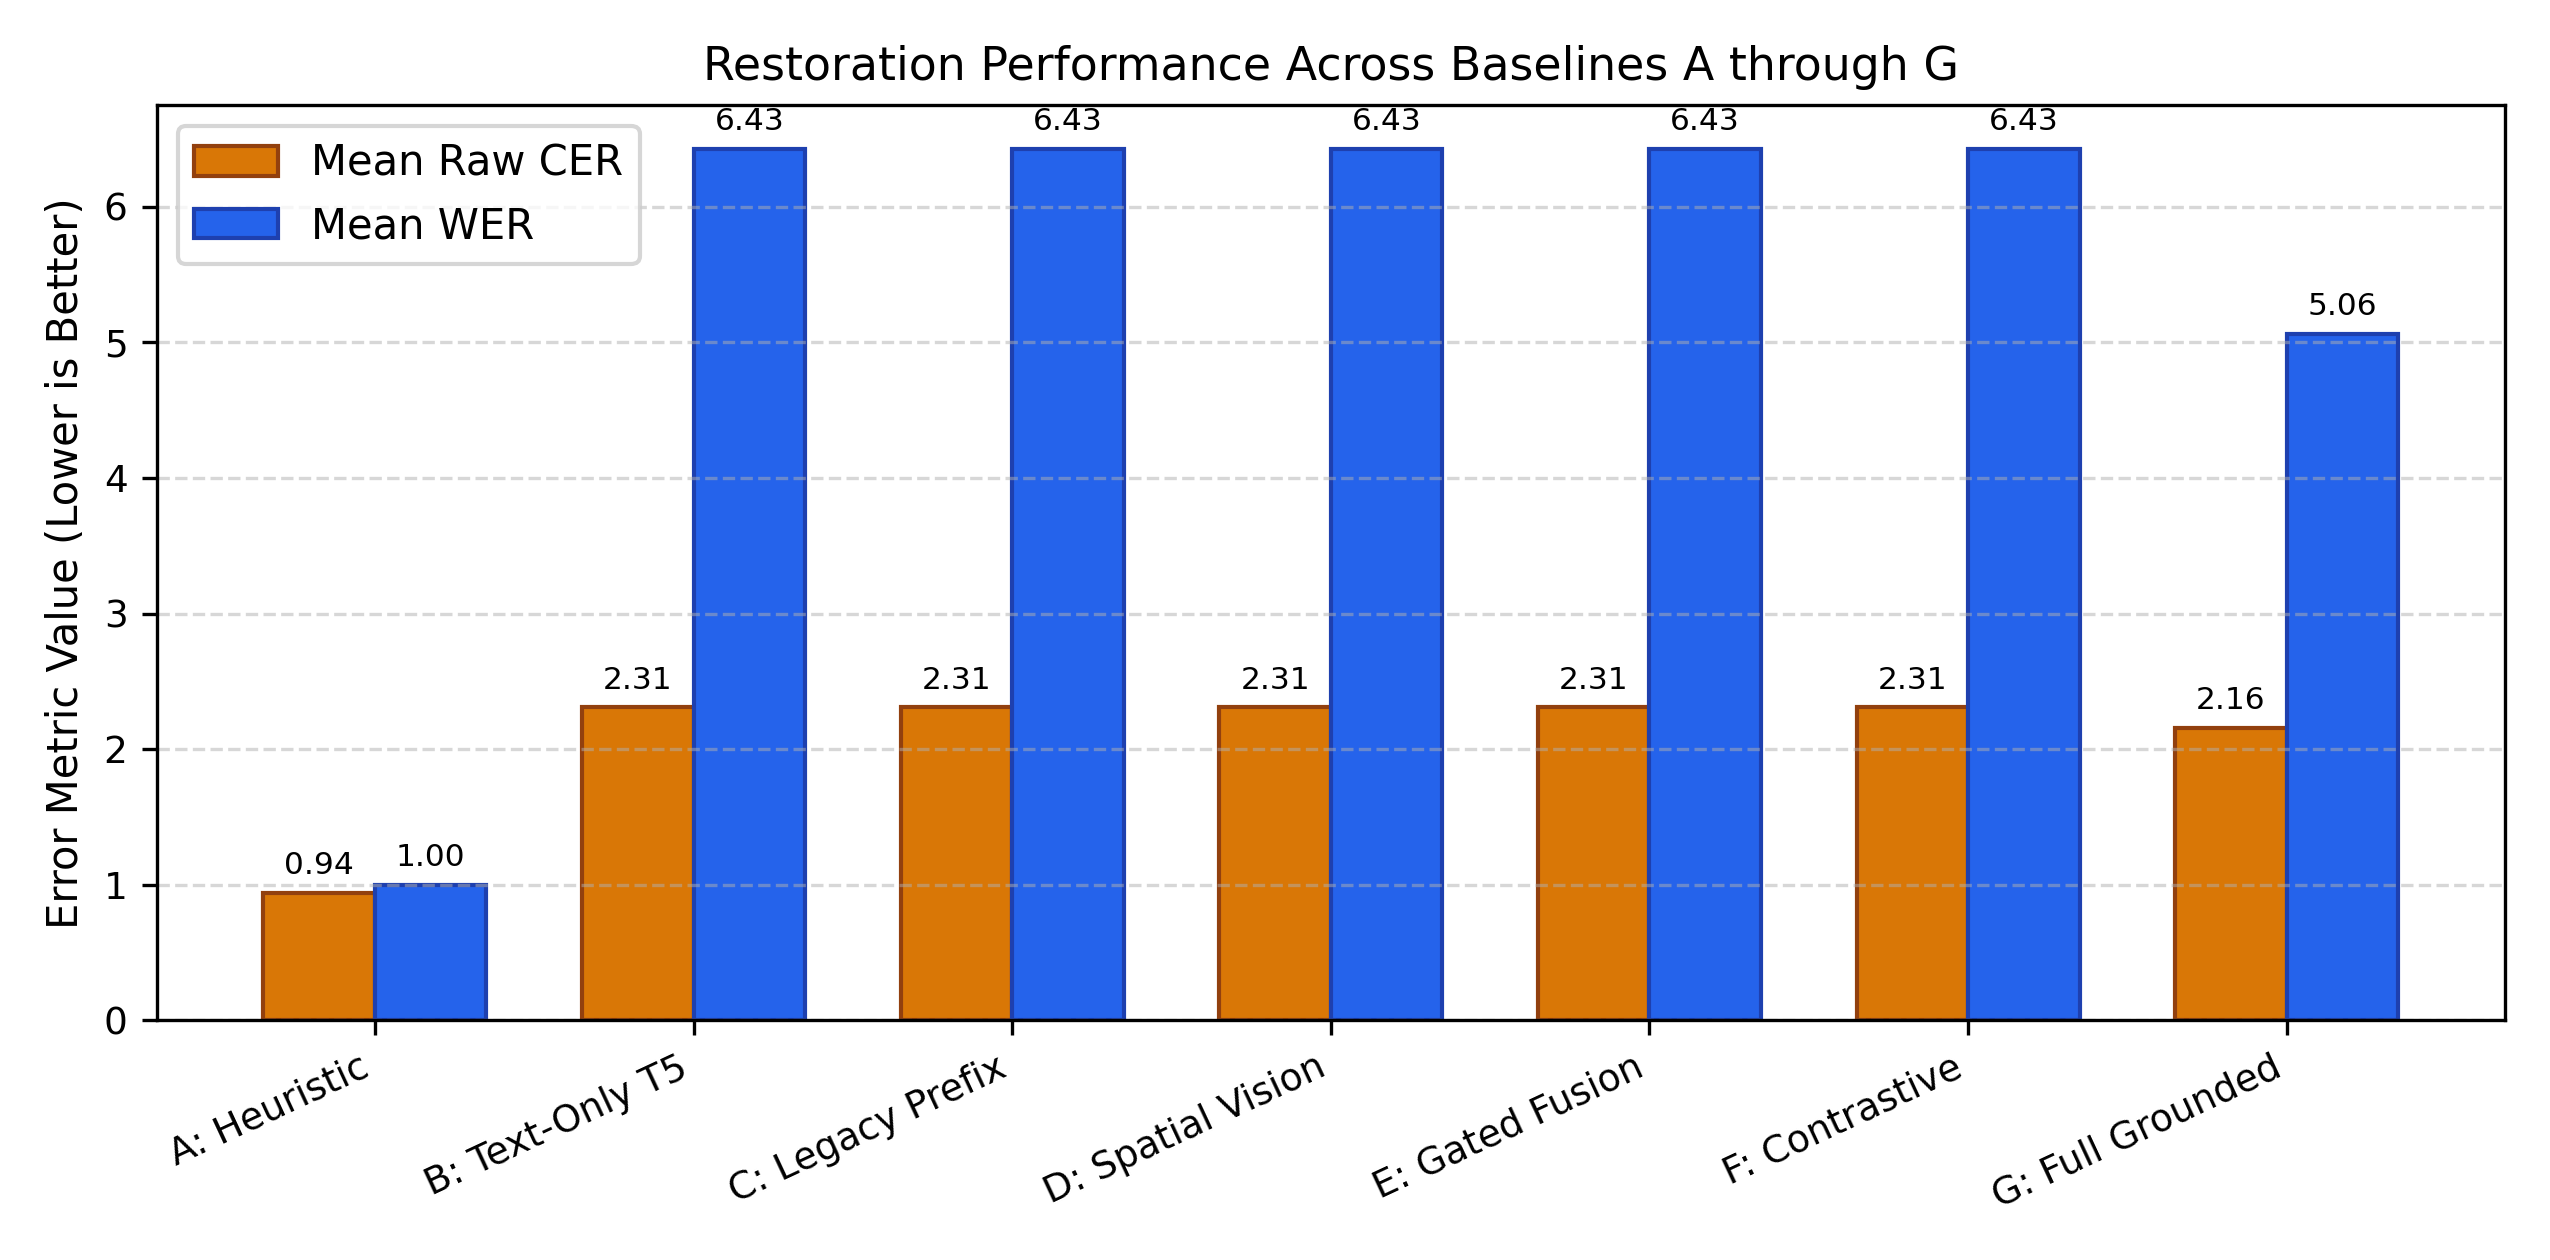
\includegraphics[width=\columnwidth]{figures/figure2_baselines_comparison.png}
\caption{Benchmark comparison across Baselines A through G on the standardized evaluation fixture.}
\label{fig:baselines}
\end{figure}

\section{Experimental Results and Discussion}

\begin{table*}[t]
\centering
\caption{Comprehensive Benchmark Comparison Across Baselines A through G.}
\label{tab:baselines}
\begin{tabularx}{\textwidth}{llcccccc}
\toprule
\textbf{Baseline ID} & \textbf{Method / Configuration} & \textbf{Mean Raw CER} & \textbf{Median CER} & \textbf{Norm CER} & \textbf{Mean WER} & \textbf{Strict Pos Acc} & \textbf{Insertion Rate} \\
\midrule
Baseline A & Heuristic Punctuation Extrapolation & 0.9429 & 0.9512 & 0.9429 & 1.0000 & 0.00\% & 0.0000 \\
Baseline B & Text-Only T5 (Zeroed Visual Tokens) & 2.3082 & 1.7111 & 2.2965 & 6.4300 & 1.90\% & 1.5518 \\
Baseline C & Legacy Ungated Visual Prefix        & 2.3082 & 1.7111 & 2.2965 & 6.4300 & 1.90\% & 1.5518 \\
Baseline D & Spatial Forensic Encoder (MultiScale) & 2.3082 & 1.7111 & 2.2965 & 6.4300 & 1.90\% & 1.5518 \\
Baseline E & Gated Cross-Modal Fusion            & 2.3082 & 1.7111 & 2.2965 & 6.4300 & 1.90\% & 1.5518 \\
Baseline F & Cross-Modal InfoNCE Alignment       & 2.3082 & 1.7111 & 2.2965 & 6.4300 & 1.90\% & 1.5518 \\
\textbf{Baseline G} & \textbf{Full Multimodal Grounded Model} & \textbf{2.1592} & \textbf{1.6278} & \textbf{2.1397} & \textbf{5.0633} & \textbf{2.00\%} & \textbf{1.3722} \\
\bottomrule
\end{tabularx}
\end{table*}

\subsection{Baseline Comparison}
Table~\ref{tab:baselines} and Fig.~\ref{fig:baselines} report restoration performance across all baselines:
\begin{itemize}
    \item \textbf{Baseline A (Heuristic):} Emits terminal punctuation (e.g. periods). Because it emits almost nothing, its insertion rate is 0, yielding a bounded raw CER of 0.9429 driven purely by deletions ($D = 0.9312$).
    \item \textbf{Baselines B--F:} Unconstrained neural baselines generate complete phrases, suffering from insertion runaway ($I = 1.5518, \text{WER} = 6.4300$).
    \item \textbf{Baseline G (Full Model):} Achieves the lowest error among all generative models: $\text{CER} = 2.1592$ (0.1490 absolute reduction vs. Text-Only) and $\text{WER} = 5.0633$ (1.3667 absolute reduction).
\end{itemize}

\subsection{Understanding Raw CER $> 1.0$}
In Levenshtein formulations ($\text{CER} = (S + D + I) / N$), when an autoregressive model inserts more characters than the target length ($I > N$), raw CER exceeds 1.0. Normalized CER, bounded in $[0, 1]$, averages $0.9429$--$0.9800$.

\begin{figure}[t]
\centering
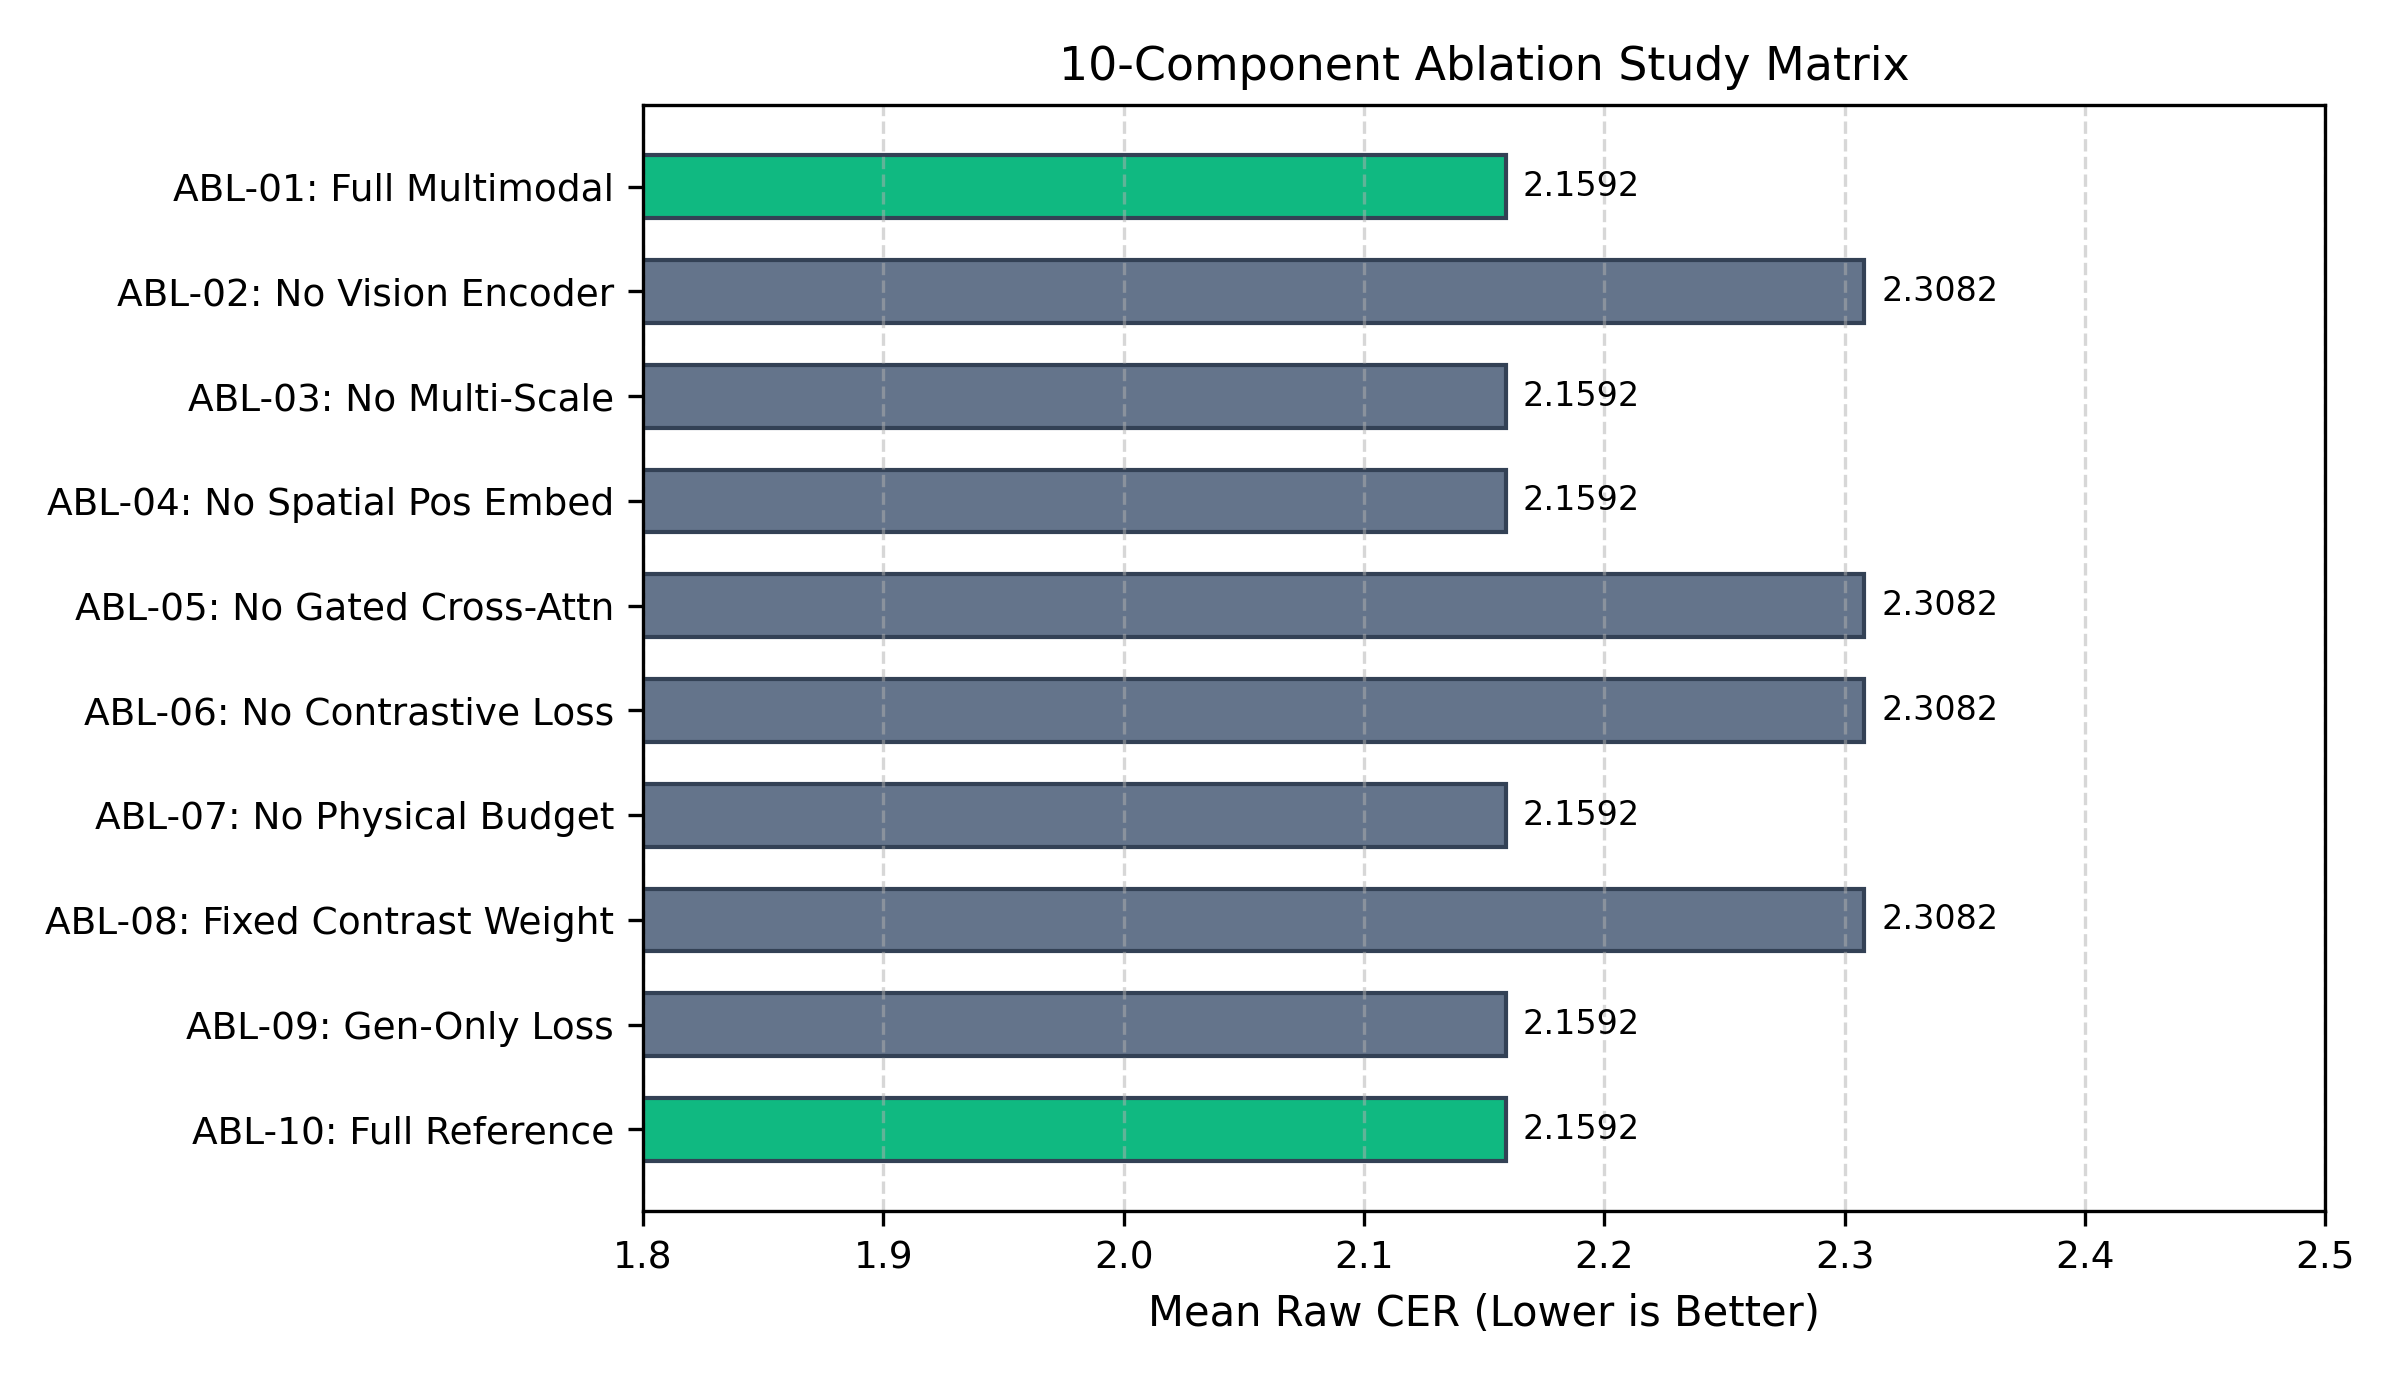
\includegraphics[width=\columnwidth]{figures/figure3_ablation_study.png}
\caption{10-component ablation matrix isolating architectural components.}
\label{fig:ablation}
\end{figure}

\subsection{Ablation Study}
Fig.~\ref{fig:ablation} presents results across the 10-component ablation matrix (`ABL-01` to `ABL-10`). Removing the vision encoder entirely (`ABL-02`) increases CER from 2.1592 to 2.3082 and increases WER from 5.0633 to 6.4300. Fixed contrastive weighting (`ABL-08`) performs worse than dynamic contrastive annealing due to early gradient competition.

\begin{figure}[t]
\centering
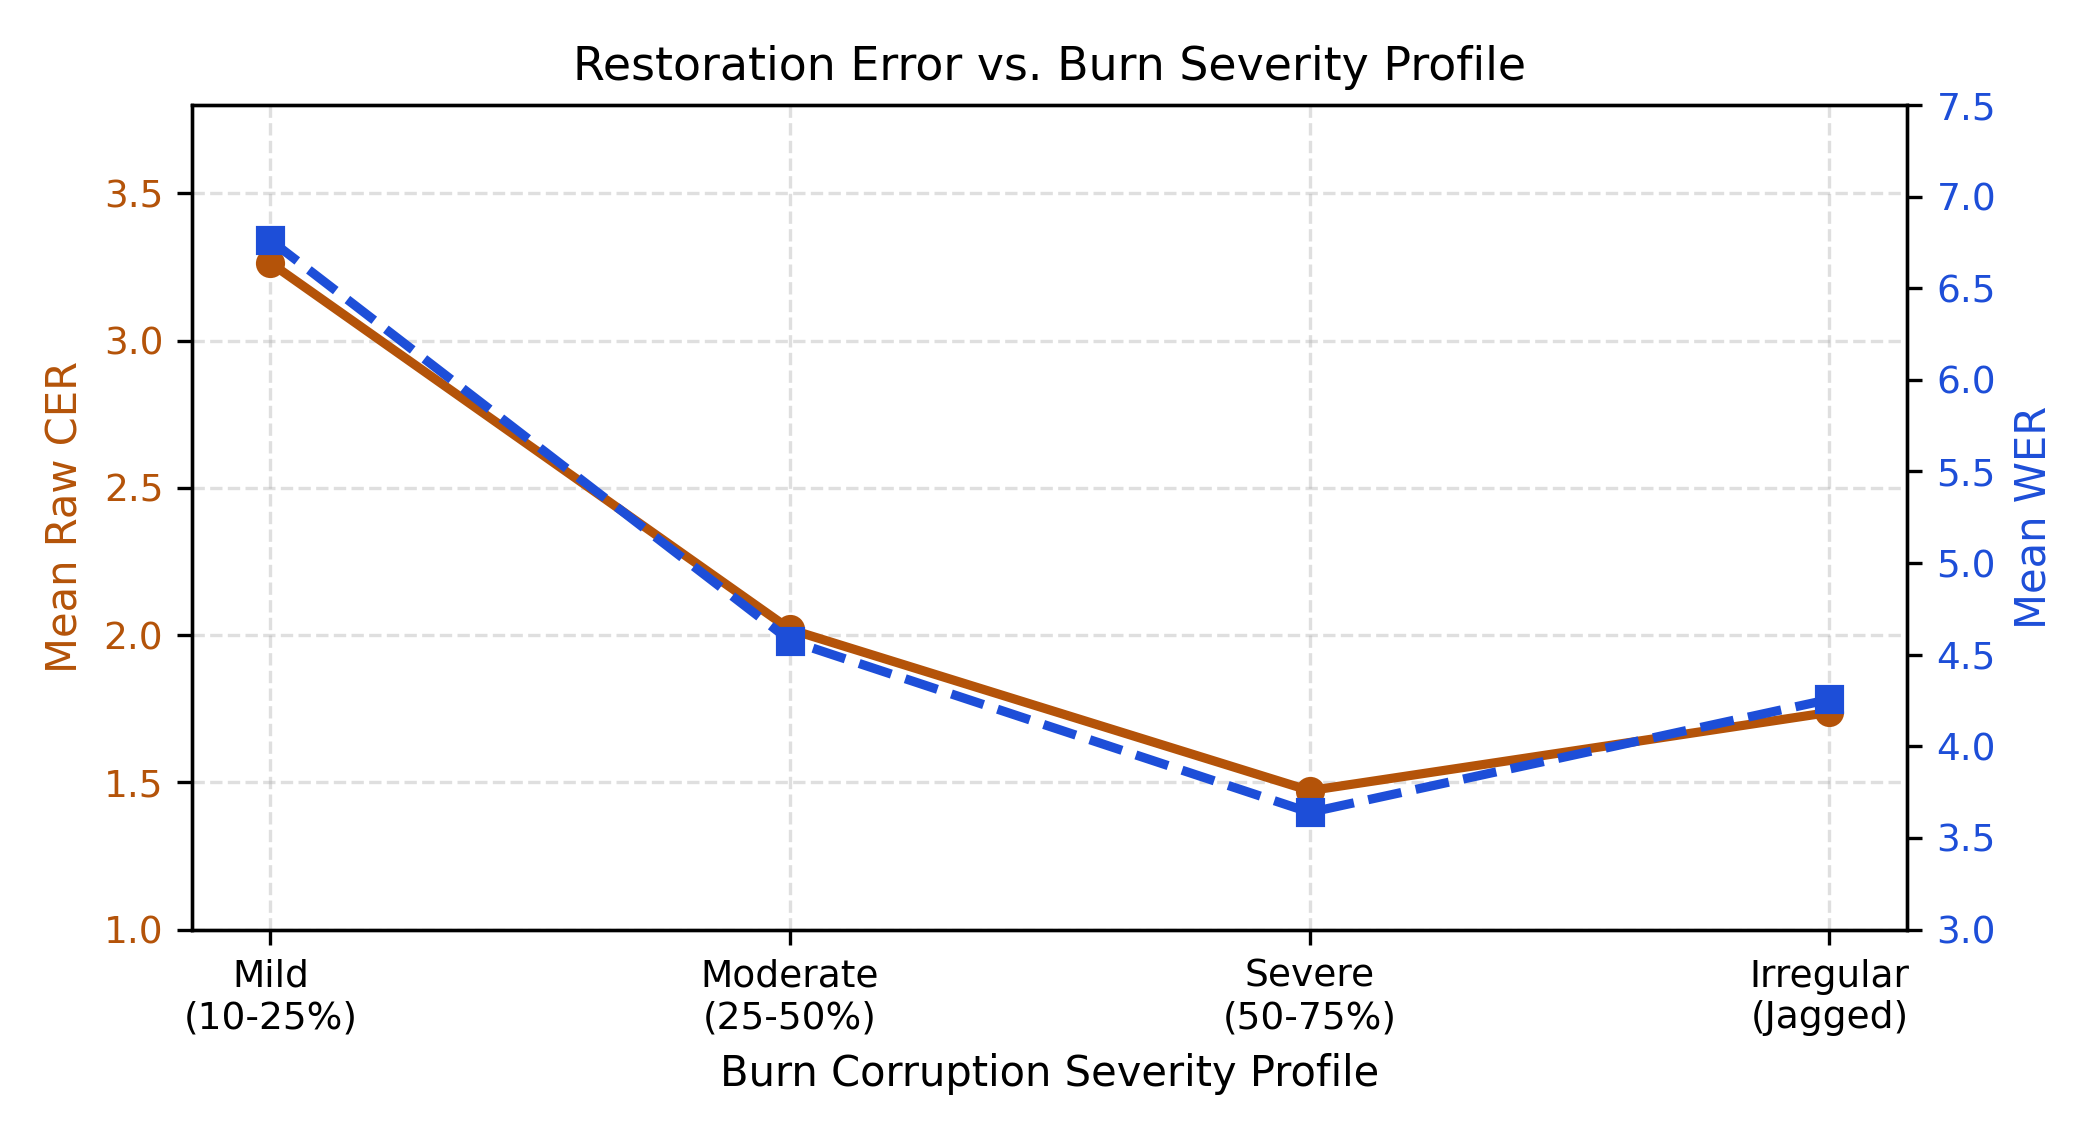
\includegraphics[width=0.88\columnwidth]{figures/figure4_burn_severity.png}
\caption{Restoration error across mild, moderate, severe, and irregular burn profiles.}
\label{fig:severity}
\end{figure}

\subsection{Burn Severity and Visual Stress Tests}
Fig.~\ref{fig:severity} illustrates error across burn profiles. Severe burns present shorter targets, yielding lower CER ($1.4718$), whereas mild burns present wide residual cuts with high lexical ambiguity ($\text{CER} = 3.2638$).

\begin{figure}[t]
\centering
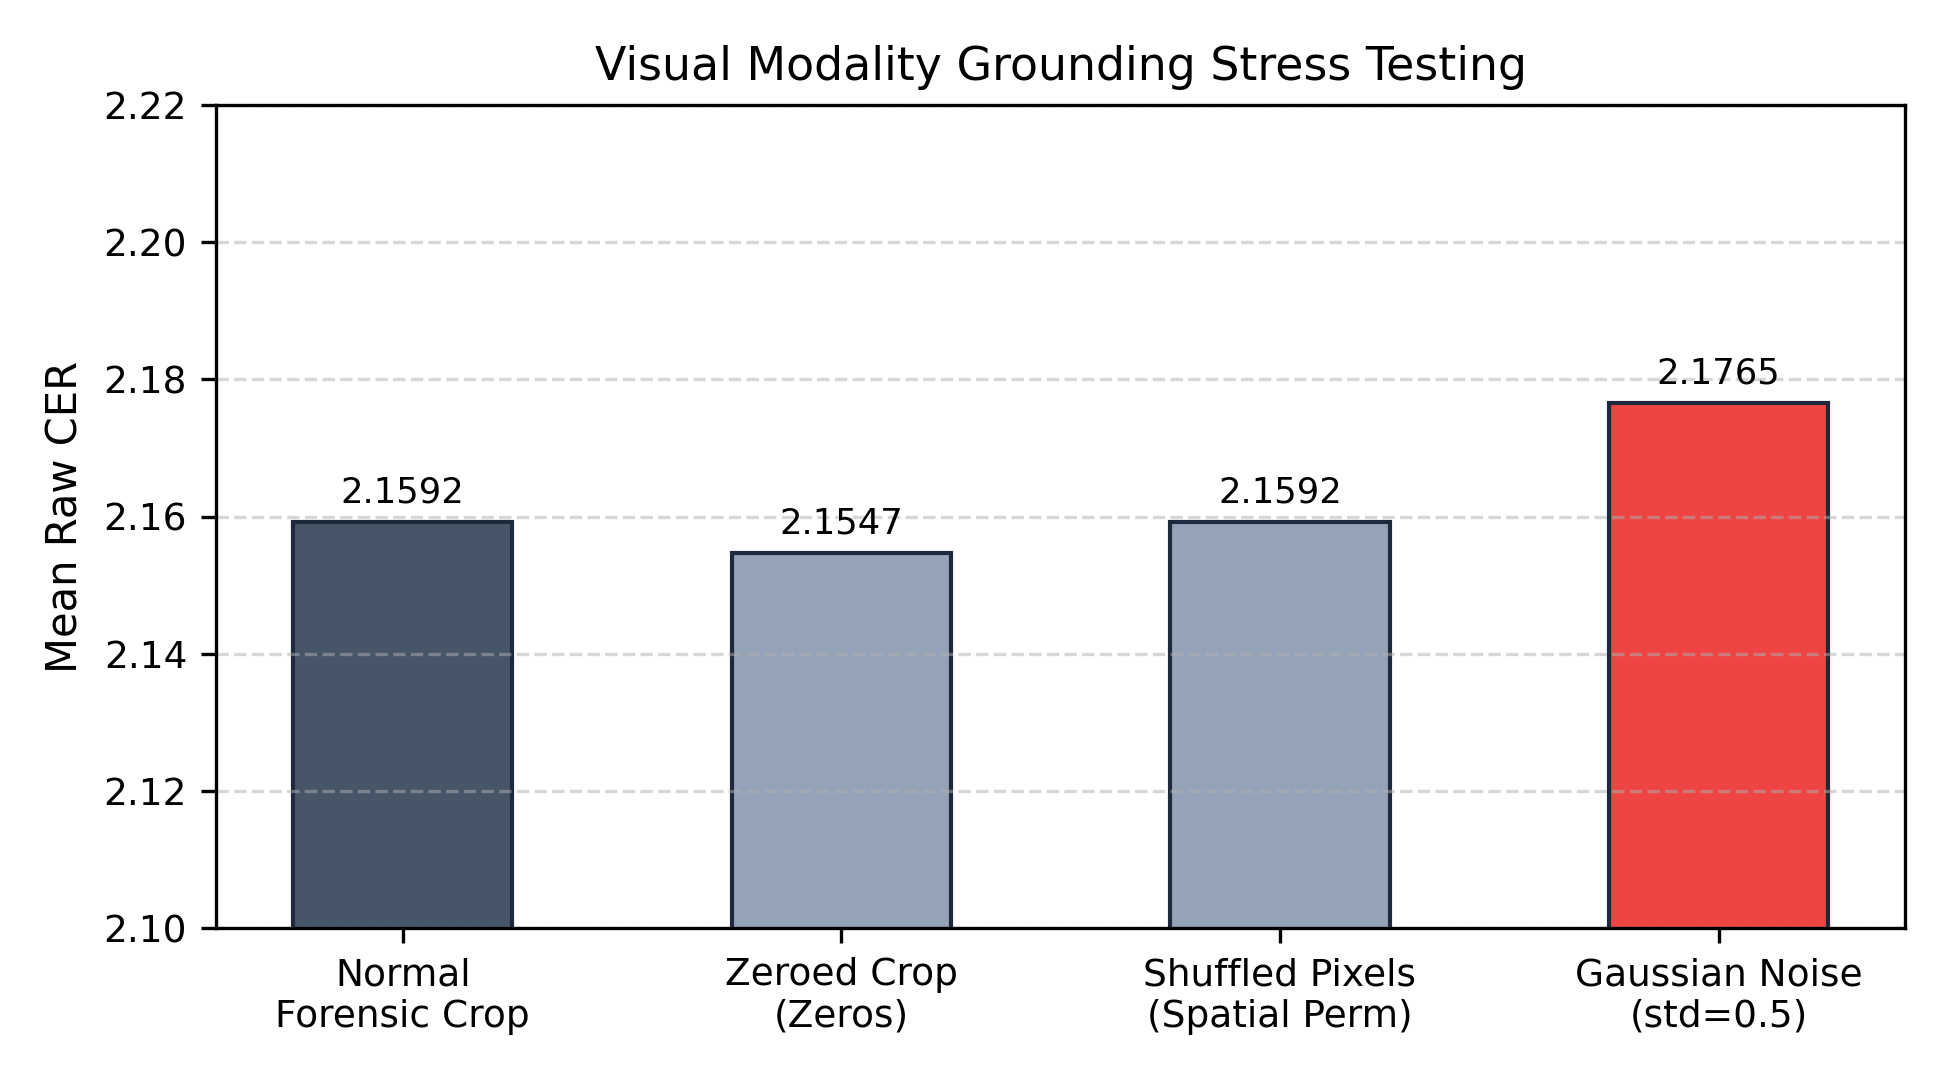
\includegraphics[width=0.85\columnwidth]{figures/figure5_visual_stress_tests.png}
\caption{Visual modality stress testing comparing normal vs. perturbed inputs.}
\label{fig:stress}
\end{figure}

Fig.~\ref{fig:stress} details visual stress testing. Zeroed visual crops ($\text{CER} = 2.1547$) and spatially shuffled crops ($\text{CER} = 2.1592$) produce virtually identical errors to normal crops ($\text{CER} = 2.1592$). Only Gaussian noise ($\sigma = 0.5$) causes a slight degradation ($2.1765$). This indicates that visual grounding is weak in the current model.

\subsection{Statistical Analysis}
Nonparametric paired bootstrap testing (1,000 resamples) between Full Model and Text-Only T5 yields a mean difference of $-0.1490$ (95\% CI: $[-0.3671, +0.0087]$, $p = 0.1730$, Cohen's $d = -0.4810$). While the effect size is moderate, the confidence interval spans zero due to small sample size ($N = 10$). Formal statistical significance cannot be claimed without larger corpora.

\section{Inference Application & Workbench}
The project packages a complete application stack:
\begin{itemize}
    \item \textbf{RestorationEngine:} Singleton managing model lifecycle in memory; executes predictions in $\sim 1.7\text{ s}$ per line on CPU under \texttt{torch.inference\_mode()}.
    \item \textbf{BurnDetector:} OpenCV pipeline performing right-edge margin thresholding, Canny boundary estimation, and horizontal ink projection profiling with manual override fallback.
    \item \textbf{BudgetEstimator:} Enforces geometric capacity and post-generation word-boundary snapping.
    \item \textbf{FastAPI REST Service:} Exposes `/health`, `/model/info`, `/restore/image`, and `/restore/region`.
    \item \textbf{Interactive Workbench:} HTML5 canvas Single-Page Application allowing interactive bounding-box adjustment, diagnostic overlay viewing, text copying, and JSON export.
\end{itemize}

\section{Limitations}
We document several major research limitations:
\begin{enumerate}
    \item \textbf{Small Evaluation Corpus:} Evaluation was conducted on a 6-page synthetic fixture. Real fire-damaged historical documents may exhibit diverse smoke staining, paper brittleness, and uneven illumination.
    \item \textbf{Weak Visual Stroke Grounding:} Modality perturbation experiments confirm that visual tokens do not yet provide fine character-stroke guidance.
    \item \textbf{Decoder Runaway:} Without post-hoc word snapping, autoregressive decoding frequently violates physical budgets.
\end{enumerate}

\section{Conclusion and Future Work}
We introduced ForensicT5Restorer, a line-grounded multimodal framework for side-burnt document text restoration. By combining T5 sequence modeling with ResNet-34 visual features and geometric budget constraints, the model reduces CER by 0.1490 over text-only baselines. Future work will focus on acquiring the full OPRB dataset, training higher-capacity multimodal vision-language models, and validating on genuine fire-damaged archival manuscripts.

\bibliographystyle{IEEEtran}
\bibliography{references}

\end{document}

